\section{Popis optimalizačního rámce}\label{ramec}
Pro použití popsaných optimalizačních metod v rámci problematiky dynamiky tekutin a numerických simulací je potřeba vytvořit plně automatizovaný optimalizační rámec. Je vhodné navrhnout takový rámec, jehož jednotlivé části budou dostatečně modulární, tedy v případě potřeby může být pro vykonání specifického úkonu v rámci procesu optimalizace snadno použita jiná metoda. Celkový navržený rámec zahrnuje několik částí, které dále popíšeme:

\begin{enumerate}
	\item \textit{Optimalizace}: První část zahrnuje samotnou použitou optimalizační metodu, která řídí celý další proces. V této části je definována řešená úloha společně s případnými požadovanými vazbami. Jak již bylo zmíněno, je vhodné, aby tato část byla co nejvíce nezávislá na ostaních částech popisovaného optimalizačního rámce. To nám dovolí použít různé metody implementované v jiných programovacích jazycích bez narušení chodu celkového procesu.
	
	V této práci budeme pracovat s metodami L-BFGS (viz sekce \ref{BFGS}) a Nelderovou-Meadovou metodou (viz sekce \ref{heuristic}). Pro implementeci obou těchto metod použijeme volně dostupný balík \texttt{Optim.jl} \cite{Optim.jl} implementovaný v programovacím jazyce Julia. Pro zahrnutí vazeb použijeme v obou případech metodu transformující účelovou funkci na extrémní bariérovou funkci, která byla pro účely této práce implementována nad rámec použitého balíku. Pro výpočet gradientu v rámci metody L-BFGS použijeme automatickou diferenciaci, která je dostupná v rámci balíku \texttt{Optim.jl} a jejíž detaily jsou popsány v \cite{Optim.jl}. Metodu L-BFGS s toutou volbou výpočtu gradientu budeme dále značit L-BFGS(A).
	
	Dále v rámci optimalizačního rámce zařazujeme metodu přímého vyhledávání MADS (viz sekce \ref{direct-search}) implementovanou v programovacím jazyce C++ ve volně dostupné knihovně \texttt{NOMAD} \cite{nomad}. Pro zarhnutí vazeb rovněž použijeme extrémní bariérovou funkci, která je v případě knihovny \texttt{NOMAD} její součástí. Podotkněme, že v rámci této práce metoda MADS není využita.
	
	\item \textit{Generování geometrie}: Optimalizační parametry, jejichž hodnota se v každé iteraci optimalizace mění, jsou předány do generátoru geometrie. Pro generování geometrie, která je dále využita v numerické simulaci, byl použit balík \texttt{meshgenerator} implementovaný v jazyce Python. Zmíněný balík vznikl pro účely této práce a je blíže popsán v kapitole \ref{geometrie}.
	
	\item \textit{Numerická simulace}: Poslední částí optimalizačního rámce je řešič umožňující vyčíslení optimalizované účelové funkce. V rámci této práce se zabýváme pouze problémy týkajícími se dynamiky tekutin. Pro numerickou simulaci proudění byla použita metoda LBM, která je společně s implementačními poznámkami popsána v kapitole \ref{lbm}.
	
\end{enumerate}
Schématicky je propojení jednotlivých částí optimalizačního rámce zobrazeno na obr. \ref{fig:framework}.

\begin{figure}[H]
	\vspace{8mm}
	\centering
	\includegraphics[width=0.85\textwidth]{figures/framework.pdf}
	\vspace{7mm}
	\caption{Schématické znázornění navrženého optimalizačního rámce. Šipkami je znázorněno propojení jednotlivých částí, nad šipkou je pak zdůrazněno, co jednotlivé části předávají v procesu dále.}
	\label{fig:framework}
\end{figure}